\documentclass[10pt,letterpaper]{article}
\usepackage[top=0.85in,left=2.75in,footskip=0.75in]{geometry}
\usepackage{amsmath,amssymb}
\usepackage{changepage}
\usepackage[utf8x]{inputenc}
\usepackage{textcomp,marvosym}
\usepackage{cite}
\usepackage{nameref,hyperref}
\usepackage[right]{lineno}
\usepackage{microtype}
\usepackage[table]{xcolor}
\usepackage{array}
\newcolumntype{+}{!{\vrule width 2pt}}

% create \thickcline for thick horizontal lines of variable length
\newlength\savedwidth
\newcommand\thickcline[1]{%
  \noalign{\global\savedwidth\arrayrulewidth\global\arrayrulewidth 2pt}%
  \cline{#1}%
  \noalign{\vskip\arrayrulewidth}%
  \noalign{\global\arrayrulewidth\savedwidth}%
}

% \thickhline command for thick horizontal lines that span the table
\newcommand\thickhline{\noalign{\global\savedwidth\arrayrulewidth\global\arrayrulewidth 2pt}%
\hline
\noalign{\global\arrayrulewidth\savedwidth}}


% Remove comment for double spacing
%\usepackage{setspace}
%\doublespacing

% Text layout
\raggedright
\setlength{\parindent}{0.5cm}
\textwidth 5.25in
\textheight 8.75in

% Bold the 'Figure #' in the caption and separate it from the title/caption with a period
% Captions will be left justified
\usepackage[aboveskip=1pt,labelfont=bf,labelsep=period,justification=raggedright,singlelinecheck=off]{caption}
\renewcommand{\figurename}{Fig}

% Use the PLoS provided BiBTeX style
\bibliographystyle{plos2015}

% Remove brackets from numbering in List of References
\makeatletter
\renewcommand{\@biblabel}[1]{\quad#1.}
\makeatother



% Header and Footer with logo
\usepackage{lastpage,fancyhdr,graphicx}
\usepackage{epstopdf}
%\pagestyle{myheadings}
\pagestyle{fancy}
\fancyhf{}
%\setlength{\headheight}{27.023pt}
%\lhead{\includegraphics[width=2.0in]{PLOS-submission.eps}}
\rfoot{\thepage/\pageref{LastPage}}
\renewcommand{\headrulewidth}{0pt}
\renewcommand{\footrule}{\hrule height 2pt \vspace{2mm}}
\fancyheadoffset[L]{2.25in}
\fancyfootoffset[L]{2.25in}
\lfoot{\today}

%% Include all macros below

\newcommand{\lorem}{{\bf LOREM}}
\newcommand{\ipsum}{{\bf IPSUM}}

%% extra packages
\usepackage{caption}
\usepackage{subcaption}

%% END MACROS SECTION


\begin{document}
\vspace*{0.2in}

% Title must be 250 characters or less.
\begin{flushleft}
{\Large
\textbf\newline{Galaxy Training: A Powerful Framework for Teaching!} 
}
\newline
% Insert author names, affiliations and corresponding author email (do not include titles, positions, or degrees).
\\
\color{blue} \textbf{NOTE: please add your name and affiliation below if you want to be on this paper! This project is only possibly because of the amazing community behind it. If you have contributed in any way to this project, you may add yourself as an author. (And contributions come in many forms, GitHub contributions are just one form, and not a requirement). } \\
\color{black}
\ \\
Saskia Hiltemann\textsuperscript{1\Yinyang},
Helena Rasche\textsuperscript{1,15,2\Yinyang},
Simon Gladman \textsuperscript{3},
Hans-Rudolf Hotz \textsuperscript{4},
Delphine Larivière \textsuperscript{5},
Daniel Blankenberg \textsuperscript{6},
Pratik D. Jagtap \textsuperscript{7},
Thomas Wollmann \textsuperscript{8},
Anthony Bretaudeau \textsuperscript{9,10},
Nadia Goué \textsuperscript{11},
Timothy J. Griffin \textsuperscript{7},
Coline Royaux\textsuperscript{12},
Yvan Le Bras\textsuperscript{12},
Subina Mehta\textsuperscript{7},
Anna Syme\textsuperscript{3},
Frederik Coppens\textsuperscript{13,14},
Bert Droesbeke\textsuperscript{13,14},
Nicola Soranzo\textsuperscript{16},,
\color{blue}Add your name here\textsuperscript{15}\color{black},
Björn Grüning \textsuperscript{2\ddag}
Bérénice Batut\textsuperscript{2\ddag},
with the GTN community\textsuperscript{\textpilcrow}
\\
\bigskip
\textbf{1} Clinical Bioinformatics Group, Department of Pathology, Erasmus Medical Center, Wytemaweg 80, 3015 CN, Rotterdam, The Netherlands \\
\textbf{2} Bioinformatics Group, Department of Computer Science, Albert-Ludwigs-University Freiburg, Georges-Köhler-Allee 106, Freiburg 79110, Germany \\
\textbf{3} Melbourne Bioinformatics, University of Melbourne, Parkville, Victoria, Australia \\
\textbf{4} Friedrich Miescher Institute for Biomedical Research, Basel, Switzerland and SIB Swiss Institute of Bioinformatics, Basel, Switzerland \\
\textbf{5} Eberly College of Science, Pennsylvania State University, State College, U.S.A. \\
\textbf{6} Genomic Medicine Institute, Lerner Research Institute, Cleveland Clinic, Cleveland, OH, USA  \\
\textbf{7} Department of Biochemistry, Molecular Biology and Biophysics, University of Minnesota, Minneapolis, MN, USA  \\
\textbf{8} Biomedical Computer Vision Group, BioQuant, IPMB, Heidelberg University\\ Im Neuenheimer Feld 267, Heidelberg, Germany. \\
\textbf{9} IGEPP, INRAE, Institut Agro, Univ Rennes, 35000, Rennes, France.\\
\textbf{10} GenOuest Core Facility, Univ Rennes, Inria, CNRS, IRISA, 35000, Rennes, France.\\
\textbf{11} AuBi, Mésocentre, Clermont Auvergne University, 63178, Aubière, France.\\
\textbf{12} PNDB French Biodiversity e-infrastructure, UMS PatriNat, French Museum of Natural History, 29900, Concarneau, France.\\
\textbf{13} Department of Plant Biotechnology and Bioinformatics, Ghent University, Technologiepark 71, Ghent 9052, Belgium.\\
\textbf{14} VIB Center for Plant Systems Biology, Technologiepark 71, Ghent 9052, Belgium.\\
\textbf{15} Academie voor de Technologie van Gezondheid en Milieu, Avans Hogeschool, Lovensdijkstraat 63, 4818 AJ Breda, the Netherlands.\\
\textbf{16} Earlham Institute, Norwich Research Park, Norwich, NR4 7UZ, UK.\\
\color{blue}\textbf{14} AddYoursHere! Affiliation Dept/Program/Center, Institution Name, City, State, Country \color{black}\\
%TODO: add your affiliation here as needed
\bigskip

% Insert additional author notes using the symbols described below. Insert symbol callouts after author names as necessary.
%
% Remove or comment out the author notes below if they aren't used.
%
% Primary Equal Contribution Note
\Yinyang These authors contributed equally to this work.

% Additional Equal Contribution Note
% Also use this double-dagger symbol for special authorship notes, such as senior authorship.
\ddag These authors also contributed equally to this work.

% Current address notes
%\textcurrency Current Address: Dept/Program/Center, Institution Name, City, State, Country % change symbol to "\textcurrency a" if more than one current address note
% \textcurrency b Insert second current address
% \textcurrency c Insert third current address

% Deceased author note
%\dag Deceased

% Group/Consortium Author Note
\textpilcrow Membership list can be found in the Acknowledgments section.

% Use the asterisk to denote corresponding authorship and provide email address in note below.
* saskiahiltemann@gmail.com

\end{flushleft}


% Please keep the abstract below 300 words
\section*{Abstract}
There is an ongoing explosion of scientific datasets being generated, brought on by recent technological advances in many areas of the natural sciences.
As a result, the life sciences have become increasingly computational in nature, and bioinformatics has taken on a central role in research studies.
However, basic computational skills and data analysis and stewardship are still rarely taught in life science educational programs \cite{Attwood2019}, resulting in a skills gap in many of the researchers tasked with analysing these big datasets.
In order to address this skills gap and empower researchers to perform their own data analyses, the Galaxy Training Network (GTN) previously developed the Galaxy Training Platform (\url{https://training.galaxyproject.org}); an open access, community-driven framework for the collection of training materials for data analysis utilizing the user-friendly Galaxy web application as its primary data analysis platform \cite{Batut2018}.

Since its inception, this training platform has thrived, with the number of tutorials and contributors growing rapidly, and the range of topics extending beyond life sciences to include topics such as climatology, cheminformatics and machine learning.
While initially aimed at supporting researchers directly, the GTN framework has proven to be an invaluable resource for educators as well. We have focused our efforts in recent years on adding increased support for this growing community of instructors.
We have added features aimed at facilitating the use of the materials in a classroom setting, simplifying the contribution flow for new materials, and have added a set of train-the-trainer lessons.
Here, we present the latest developments in the GTN project, aimed at facilitating the use of the Galaxy Training materials by educators.


%\linenumbers

\section*{Introduction}

Education is a fundamental human right (e.g.\ the Universal Declaration of Human Rights (UDHR), the International Covenant on Economic, Social and Cultural Rights (ICESCR)).
Indicators of the achievement of education as a right are outlined in the ICESCR, and further developed into what is known as the “4 As framework” \cite{tomavsevski2001human}, which specifies Availability, Accessibility, Acceptability and Adaptability as essential metrics.
The 4 As, therefore, provide a concrete set of ideals to strive towards in any global educational endeavor.
The goals of the GTN and the Galaxy project are well aligned with the 4 As.

Galaxy \cite{Jalili2020} is an open source web-based platform for accessible, reproducible, and transparent computational research, driven by an inclusive and diverse worldwide community.
Researchers are able to access a wealth of tools ($>$8,000 tools in the ToolShed (\url{https://galaxyproject.org/toolshed/}) as of July 2021), datasets, and high-performance compute resources, through a standard web browser, without requiring informatics expertise. 
However, comprehensive training is still required to adequately understand the data analyses and to accurately interpret the results. A survey of 704 NSF-BIO-funded investigators revealed that training was the top 3 of 13 most unmet needs, above HPC/cloud facilities, workflows/pipelines analysis or storage facilities needs \cite{Barone2017}.

To address this large demand for training, the Galaxy Training Network (GTN; \url{https://training.galaxyproject.org}) was founded in 2016 to provide learners with online training materials, connect them with local trainers, and help promote open data analysis practices worldwide \cite{Batut2018}. These training materials are openly developed, maintained and community-reviewed via GitHub (\url{https://github.com/galaxyproject/training-material}). 
The materials cover an increasing spread of topical domains, such as life sciences, computational chemistry, climate sciences, data visualization, statistics, and machine learning. 
The GTN website has seen a steady increase in usage since its creation; it is visited 17,000+ times per month (Figure~\ref{fig:analytics-all-users}) with 20\% of returning users, mostly from United States (28.99\% of the visits), India (8.01\%), United Kingdom (6.40\%), Germany (6.20\%) and France (3.90\%). Since September 2018, over 1,500 individual tutorial feedback forms have been submitted with a high satisfaction rate (more than 85\% had a satisfaction rate of 4 or 5, per Figure~\ref{fig:feedback}). 

By utilizing Galaxy as its primary data analysis platform, the GTN also addresses the clear demand for easily accessible compute resources for research and training in life sciences \cite{Barone2017}.
Galaxy is an ideal platform for teaching, since it takes care of all the heavy lifting behind the scenes, such as installing software and managing the compute infrastructure, leaving learners free to focus on the scientific analysis concepts at hand, rather than on the details of the technical implementations. 
By using one of the worldwide public Galaxy servers, learners and educators alike gain free access to high-performance compute resources without any of the systems administration burden. These include the UseGalaxy.* servers with Galaxy Main (\url{https://usegalaxy.org}), Galaxy Europe (\url{https://usegalaxy.eu}), and Galaxy Australia (\url{https://usegalaxy.org.au}), but also 125+ others (\url{https://galaxyproject.org/use/}). 
Therefore, over the past years, Galaxy has become increasingly attractive as a training platform for instructors around the world (Table~\ref{fig:hub-training}). For example, between June 2018 and December 2021, Galaxy Europe server alone has been used for over 170 training events, reaching more than 5,000 students. % TODO: NUMBERS
In addition to these short-running training events, GTN tutorials have also been included as part of formal undergraduate and graduate courses (see User Stories section for more details). 
%\ref{sec:userstories} if we use numbered sections

Given this observation of the value of Galaxy and the GTN in teaching activities, we have aimed to optimize the GTN framework to support educators in the development and re-use of training materials, e.g. by integrating the FAIR principles \cite{Wilkinson2016} directly into the framework.
While this is an ongoing effort, here we present our work to bring availability, accessibility, acceptability and adaptability to bioinformatics education for trainers and learners alike.

\begin{figure}[!ht]
	\centering
	\begin{subfigure}[b]{0.45\textwidth}
         \centering
         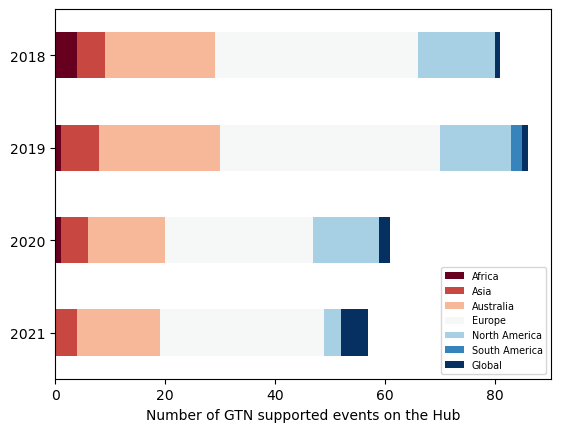
\includegraphics[width=\textwidth]{images/hub-training-per-year.png}
    \caption{Number of events per year and in total since 2018}
         \label{fig:material-evolution}
    \end{subfigure}
    \hfill
    \begin{subfigure}[b]{0.45\textwidth}
         \centering
         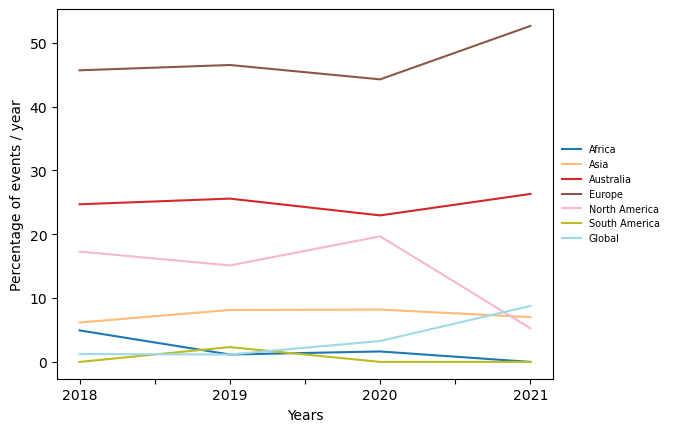
\includegraphics[width=\textwidth]{images/hub-training-over-years.png}
         \caption{Percentage of events per year for each continents (and global)}
         \label{fig:material-number}
    \end{subfigure}
	\caption{Training events supported by GTN materials, registered on the Galaxy Community Hub website (\href{https://galaxyproject.org/}{https://galaxyproject.org/}) over the last 4 years. The Jupyter notebook used to create these figures is available on the GitHub repository for this paper (\url{https://github.com/galaxyproject/GTN-community-paper-2020}) \label{fig:hub-training}}
\end{figure}

\section*{Results}

The GTN framework and community have grown significantly over the past years. In this section we describe the aims and objectives of this project, showcase some example user stories, and highlight some of the recent efforts by the GTN community to expand and improve the project. We also present how this project supports both educators and lesson developers.

%%%%%%%%%%%%%%%%%%%%%%%%%%%%%%%%%%%%%%%%%%%%%
\subsection*{GTN Overview: materials and features}
%%%%%%%%%%%%%%%%%%%%%%%%%%%%%%%%%%%%%%%%%%%%%
The GTN is continually growing, both in terms of number of tutorials as well as its community (Figure \ref{fig:material-evolution}). The GTN currently has over 230 tutorials covering 22 topics (16 scientific, 6 technical), developed by over 220 contributors (Figure~\ref{fig:material-number}).

\begin{figure}[!ht]
    \centering
    \begin{subfigure}[b]{0.4\textwidth}
         \centering
         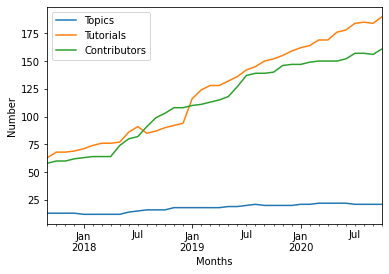
\includegraphics[width=\textwidth]{images/training-material-evolutions.png}
    \caption{Evolution of number of topics, tutorials and contributors over the months}
         \label{fig:material-evolution}
    \end{subfigure}
    \hfill
    \begin{subfigure}[b]{0.5\textwidth}
         \centering
         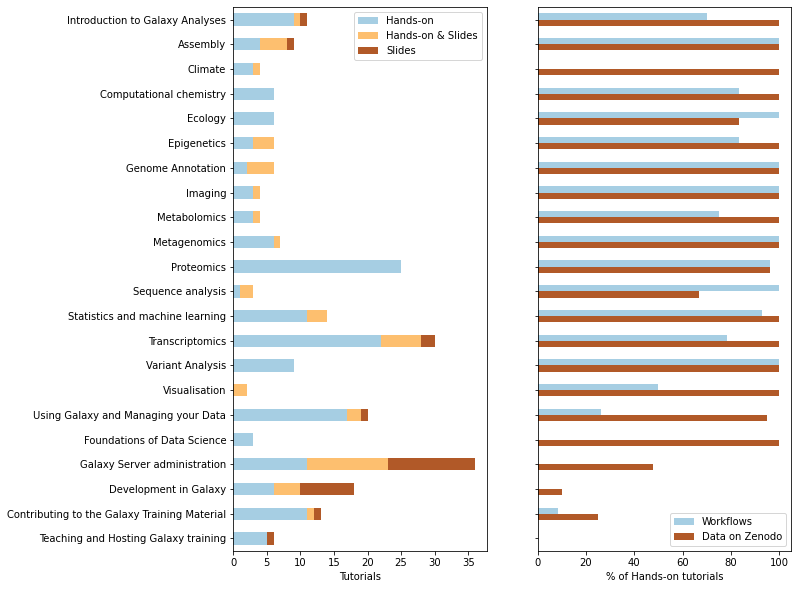
\includegraphics[width=\textwidth]{images/training-material-number.png}
         \caption{Tutorials by topics on the 7th October 2021}
         \label{fig:material-number}
    \end{subfigure}
	\caption{Numbers of tutorials, slides, hands-on tutorials and other material per topics available on the Galaxy Training Material. 
	The latest statistics are publicly available from \url{https://training.galaxyproject.org/stats}, and the Jupyter notebook used to create these figures is available on the GitHub repository for this paper (\url{https://github.com/galaxyproject/GTN-community-paper-2020})}
	\label{fig:material}
\end{figure}

Tutorials are typically constructed around a real-world \emph{research story}, e.g.\ a published journal article describing an analysis workflow or dataset. 
The tutorial starts by introducing the relevant scientific background, and then proceeds to recreate the analysis, providing details on the relevant scientific and computational concepts involved at each step. The tutorials are composed of alternating theory and hands-on sections, interspersed with formative assessment questions and exercises, and may be supported by a set of introductory slides (Figure \ref{fig:tutorial-skeleton}). Our tutorials are self-contained; everything needed to complete the tutorials is bundled with the tutorial; this includes all the datasets, lecture slides, videos, the workflows, and the list of public Galaxy servers supporting the tutorial. No software installation is needed to follow these tutorials; the only technical requirement on the learner is a web browser.

\paragraph{Automated video lectures.} In order to further increase the accessibility of our training materials, we have added support in the GTN for automatically creating videos based on lecture slide decks. The slides are narrated using automated text-to-speech (TTS), and the script is based on the speaker notes of the slides. 

\paragraph{Coding Tutorials.} In addition to analyses in Galaxy, the GTN also supports coding-oriented tutorials in the form of Jupyter notebooks and Rmarkdown. Jupyter and Rstudio can both be run within Galaxy in the form of a \emph{interactive tool}, allowing for tutorials that offer a combination of Galaxy-based analysis and coding-based R or Python analysis steps. 

\begin{figure}[!ht]
	\centering
	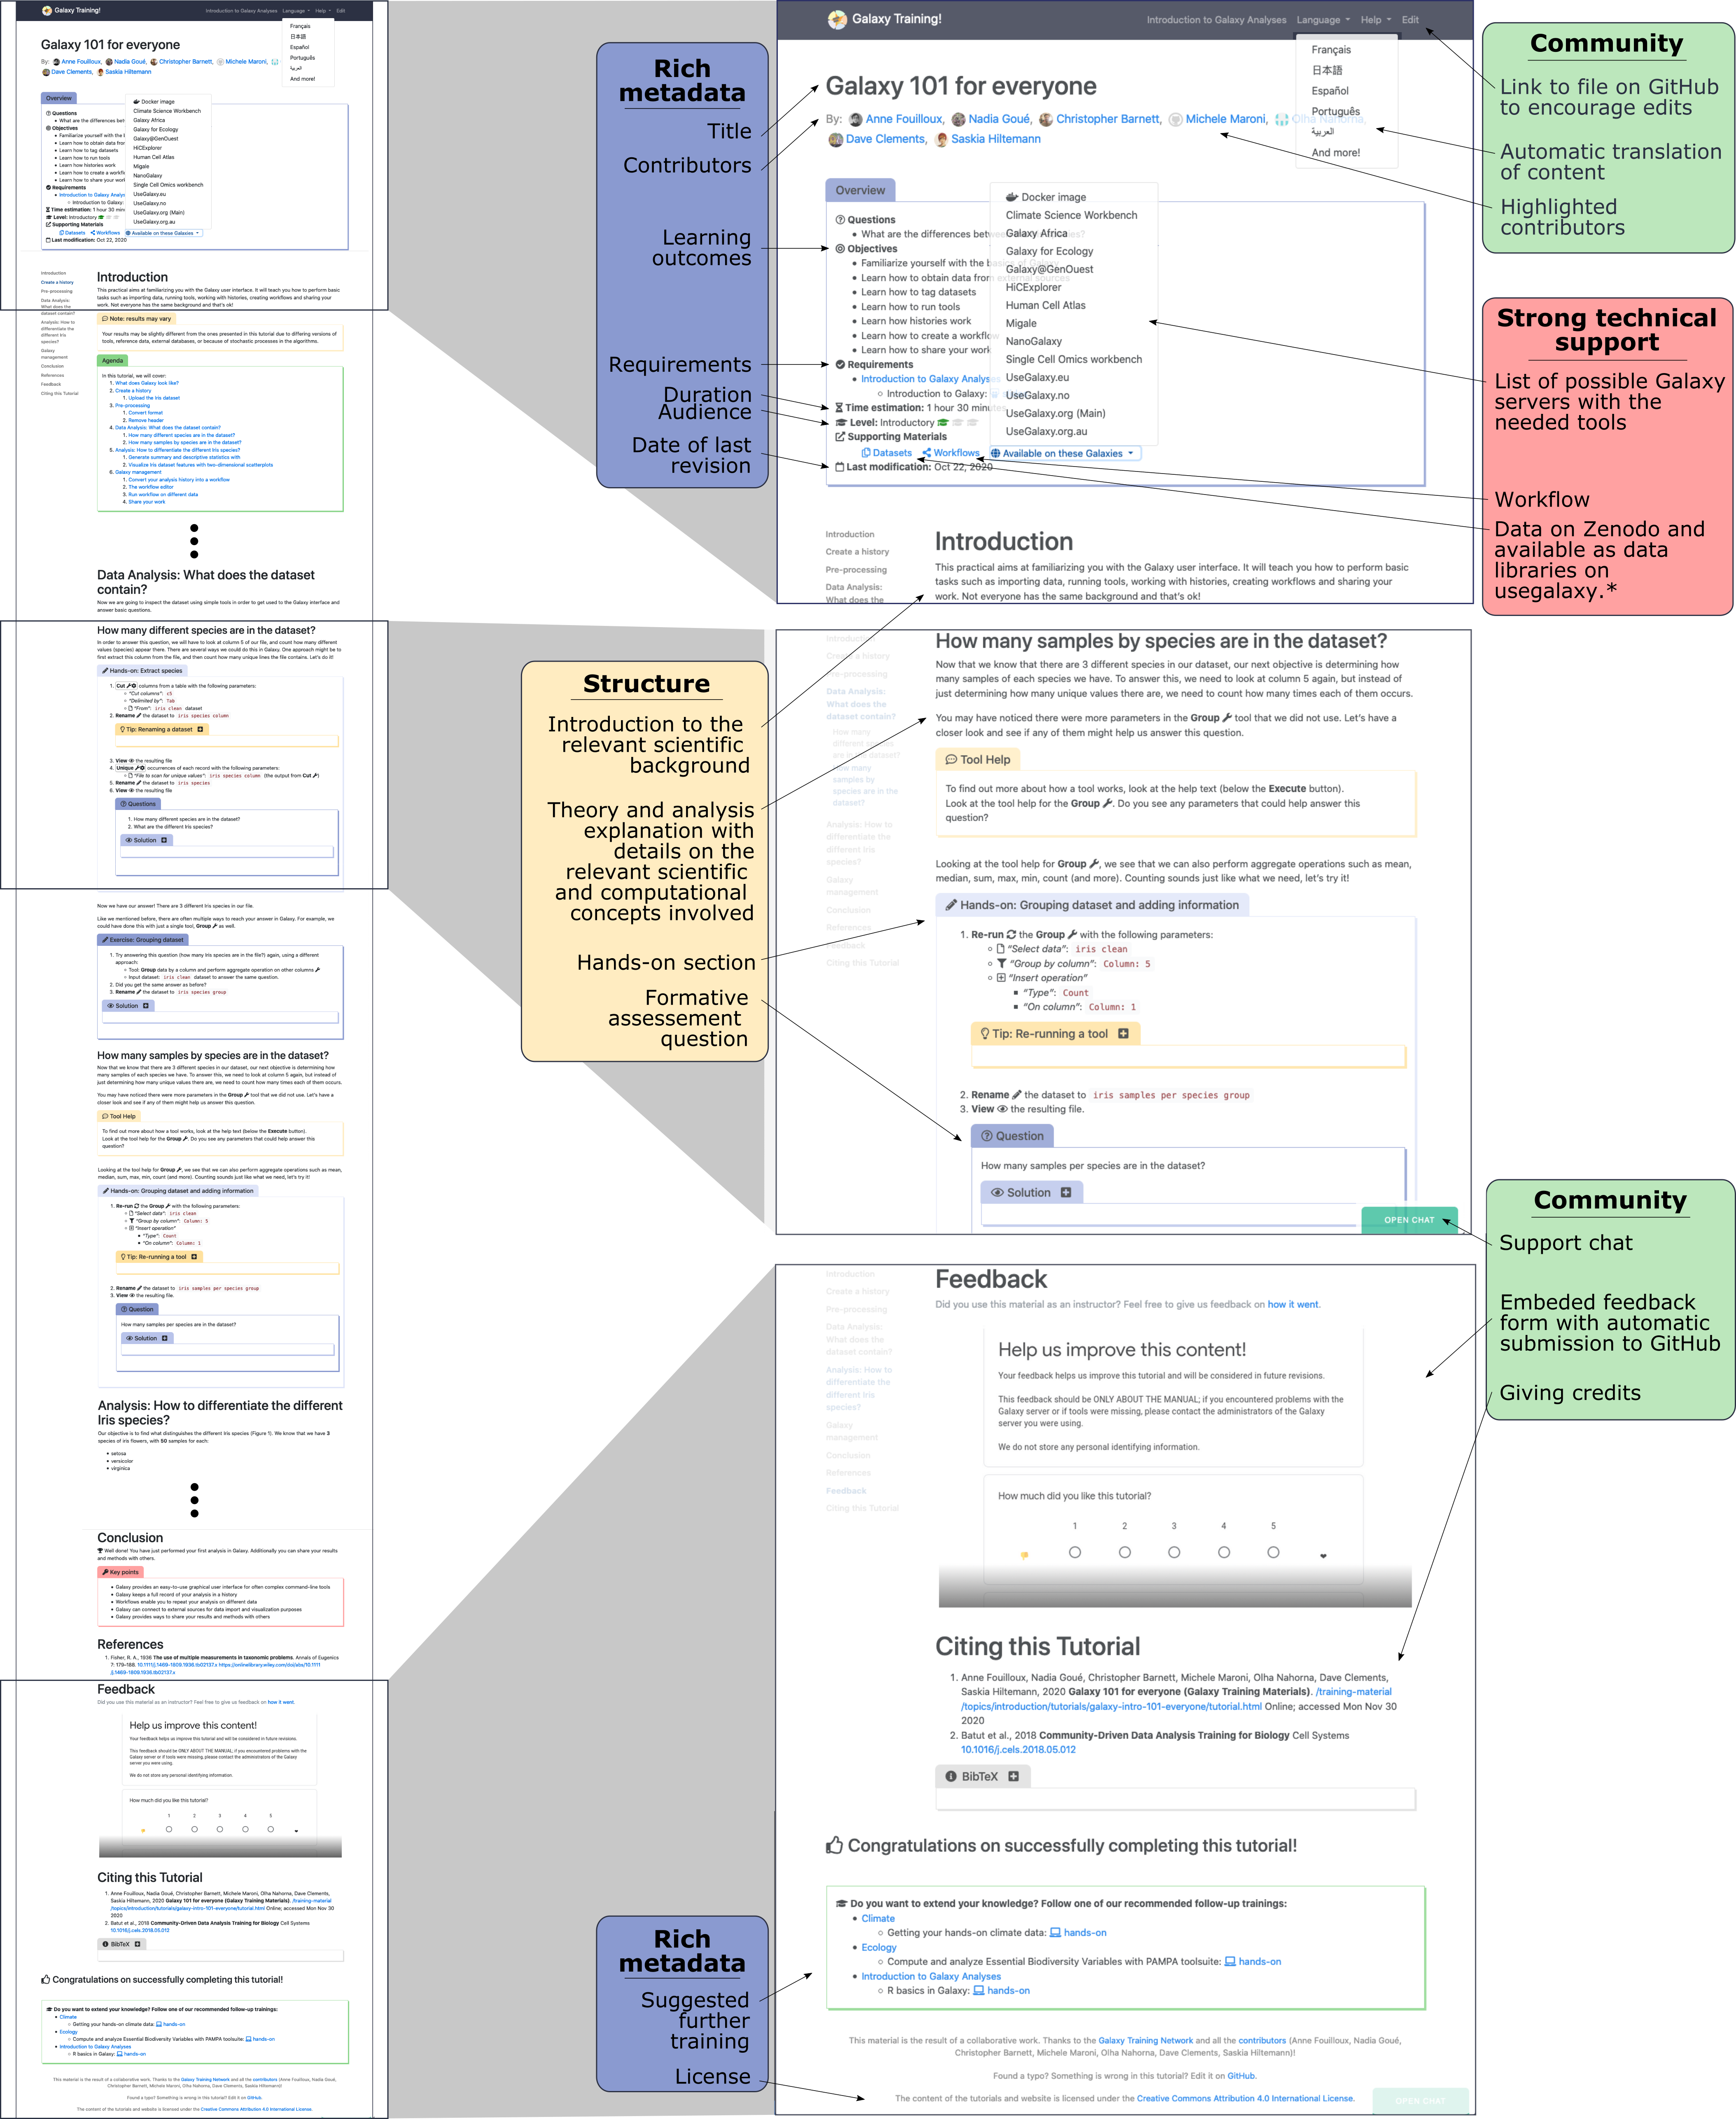
\includegraphics[width=\textwidth]{images/tutorial_skeleton.png}
	\caption{Structure of a GTN tutorial. Title and authors are listed, followed by an overview box containing metadata abot the tutorial (target audience, learning objectives, pre-requisites, supporting materials, time estimate, etc). The tutorial content itself is a mix of theory (text) and hands-on boxes describing practical steps to be performed in Galaxy. Question and answer boxes may be added at any point in the tutorial. The end of a tutorial provides a box with take-home messages, references and suggestions for further reading and follow-up tutorials. Additionally, a feedback form is embedded at the end of every tutorial. Access to support channels is provided via the top menu of the webpage. 
	\label{fig:tutorial-skeleton}}
\end{figure}

The GTN infrastructure has been developed in accordance with the FAIR (Findable, Accessible, Interoperable, Reusable) principles for training materials \cite{Garcia2020} (Table~\ref{tbl:rulesforfair}). Following these principles enables trainers and trainees to find, reuse, adapt, and improve the available tutorials. 


%%%%%%%%%%%%%%%%%%%%%%%%%%%%%%%%%%%%%%%%%%%
\subsection*{GTN for Educators}
%%%%%%%%%%%%%%%%%%%%%%%%%%%%%%%%%%%%%%%%%%%
The GTN training platform helps minimize the amount of time and effort required for instructors to prepare for and run their training courses and workshops. 

\subsubsection*{Train-the-trainer (TtT) Tutorials}
To support teachers and trainers, we have developed a dedicated topic in the GTN for TtT tutorials, covering all aspects of using the GTN materials in education. This includes best practices providing technical and logistic recommendations, accessible on the website with a series of tutorials (available in ``Teaching and Hosting Galaxy training'' category). For first-time instructors, The Galaxy Training Network has come together to collect different instructor’s experiences (``Training Philosophies'', \url{https://training.galaxyproject.org/topics/instructors/philosophies/}).

\paragraph{Preparing a Workshop.} During preparation of a workshop, organisers and instructors work together to identify relevant training materials for their event. Our training material is roughly divided into topics such as \emph{Transcriptomics} or \emph{Climate Science} on \url{https://training.galaxyproject.org}, and a search funtion is available on the GTN website. Within topics, multiple hands-on tutorials can be found - each with different stories. Each tutorial starts with a list of metadata such as pre-requisites, time estimate, questions addressed by the tutorial, as well as learning objectives following Bloom’s taxonomy \cite{Bloom1956} (Figure \ref{fig:tutorial-skeleton}). This enables instructors to identify the best tutorials for their audience. Re-usable slide decks with speaker notes are also available to introduce the topics prior to a hands-on tutorial. 

By their hands-on nature, the tutorials rely on some datasets (included in the tutorial metadata), and tools which the GTN analyses in order to list compatible public Galaxy servers. Automated workflow testing (\url{https://github.com/usegalaxy-eu/workflow-testing/}) provides reassurances to instructors, letting them know that a given tutorial will work on their selected server.

We have added support for FAQs to be added to tutorials, in order to help instructors prepare their lesson. These FAQs can be added by any community member, and typically cover common questions or frequently observed mistakes encountered during a particular tutorial.

\paragraph {Teaching the workshop.} During the workshop, instructors can introduce the topic using the available slide decks, supported by detailed speaker notes. After this theoretical introduction, instructors may either use a \emph{live-demo} approach, guiding students through the tutorials in a step-by-step fashion, or alternatively let students work through the tutorials at their own pace while providing support. The tutorials are a fully self-contained teaching resource as described in Figure \ref{fig:tutorial-skeleton}, and therefore support both these training modalities. 

A major challenge in workshop organisation is the identification of affordable and reliable compute infrastructure. The needs of training infrastructure are significantly different from regular research; analysis steps must complete in relatively short time periods in order not to disrupt the flow of the lesson. The GTN uses small (sub-sampled) training datasets for tutorials in order to reduce the run time of analysis step, but a second factor to consider are the queue times of the compute infrastructure. 
In order to support training events, Galaxy Europe developed Training Infrastructure as a Service (TIaaS) \cite{Rasche2020}. This free service provides a dedicated job queue for the participants of training events, in order to reduce queue times on the cluster and ensure courses run smoothly and efficiently. Furthermore, the TIaaS infrastructure also provides instructors with a dashboard, enabling them to monitor the progress of participants (Fig \ref{fig:tiaas-dashboard}). 
TIaaS has proven to be an excellent solution to the training infrastructure problem (Figure~\ref{fig:tiaas}) as trainers can obtain all of the benefits of a large, managed service such as scalability and on-call support. The centralisation of administration means less duplication of effort, and it has been shown to scale well whilst not exerting undue pressure on administrators of existing Galaxy servers. To date, TIaaS has been widely used: $>8000$ students taught over 229 events between 2018-06-20 and 2021-11-29, with 64\% using the GTN materials. \textbf{TODO: Update numbers + Include AU, there's another TWO THOUSAND students there.}

\begin{figure}[!ht]
	\centering
	\includegraphics[width=0.8\textwidth]{images/tiaas.png}
	\caption{The dashboard provides anonymised observability into class progress, trainers can see at a glance how many participants have completed certain steps in the tutorial, or for example quickly see which steps have led to mistakes for many participants, and may benefit from more detailed explanation in the classroom. \label{fig:tiaas-dashboard}}
\end{figure}




\subsubsection*{Feedback from Instructors}

In January 2020, we conducted a survey asking how trainers used the available training material. We received answers from 33 trainers, 88\% of which had conducted a training event in the last 3 years.
This sample consisted of a continuum of trainers, from occasional to seasoned trainers. 24\% of trainers gave a training session once in the past 3 years, and 34\% gave 10 or more training sessions, with 10\% more than 25.
Concerning the use of training materials, 79\% of them used GTN resources, and some even developed new GTN materials for the occasion. 
The participating instructors gave 4 or 5 star ratings (within a 1 to 5 scale) to the GTN tutorials, with 91\% of respondents indicating they would absolutely recommend them, confirming the satisfaction scores in the embedded feedback form (Figure~\ref{fig:feedback}).

In addition to the training material, trainers sometimes use resources for enrollment forms and certifications, or add exercises.
Trainers report the need of a few weeks to prepare new material.
This time is reduced to a couple of days when the material already exists in the GTN.
They appreciate that the GTN material is “up-to-date”, stable, and that the community provides a wide variety of analysis relevant to current research.
The trainings are “easy to follow”, have a “great pedagogy” and allow trainees to be “involved in learning”.
The use of GTN material allows them to have more time to focus on the fundamental principles of  analyses and the specific needs of the trainees.

The surveyed trainers all gave training on -omics analyses.
These trainer profiles could evolve with the introduction of training on diverse fields of expertise. In addition to hands-on and slides material, used by respectively 100\% and 72\% of the surveyed, users took advantages of the GTN materials to populate Galaxy instances with relevant tools and/or data (29\% and 38\% respectively).
Some trainers also made use of the extra material on teaching and workshop hosting (24\%) or on training philosophies (10\%) to inform and improve their training events.
The main Galaxy platforms used during these events were Galaxy Europe, Galaxy  Australia, and temporary cloud servers. Trainers also used local Galaxy instances (from their country) and  private servers (from their institution).
59\% of them relied on TIaaS (Training Infrastructure as a Service). Its usage was highly rated (100\% 5 stars) and highly recommended (94\% 5 stars).

69\% of the surveyed trainers are contributors to the training material, and among those who are not, 55\% declare planning to become one in the future.



%%%%%%%%%%%%%%%%%%%%%%%%%%%%%%%%%%%%%%%%%%%%%
\subsection*{Contributing to the GTN}
%%%%%%%%%%%%%%%%%%%%%%%%%%%%%%%%%%%%%%%%%%%%%

The GTN framework also aims to ease the burden of tutorial development, contribution and maintenance by offering a diverse set of tools and standards for tutorial authors. 

\subsubsection*{Tutorials about Contributing}

To get acquainted with the tutorial development process, the contributor starts by consulting a set of dedicated tutorials in the \emph{Contributing} topic in the GTN. These tutorials provide a step-by-step guide to creating a tutorial in the GTN framework, covering everything from technical guides concerning the framework to pedagogical best practices and submission of tutorials to GitHub.

Figure \ref{fig:contributing} depicts the typical process a tutorial contributor will go through when developing a new tutorial. The first step is usually to develop the analysis workflow in Galaxy. The next challenge is to identify or create suitable input datasets. The selected data must be informative enough to illustrate the meaning a given analysis, but not so large as to require long waiting times for upload or processing during a training event. The selected data could be a toy dataset created from scratch, or (preferably) an informative subset of a real-life dataset, for example using a single chromosome of a whole-genome dataset.

\begin{figure}[!ht]
	\centering
	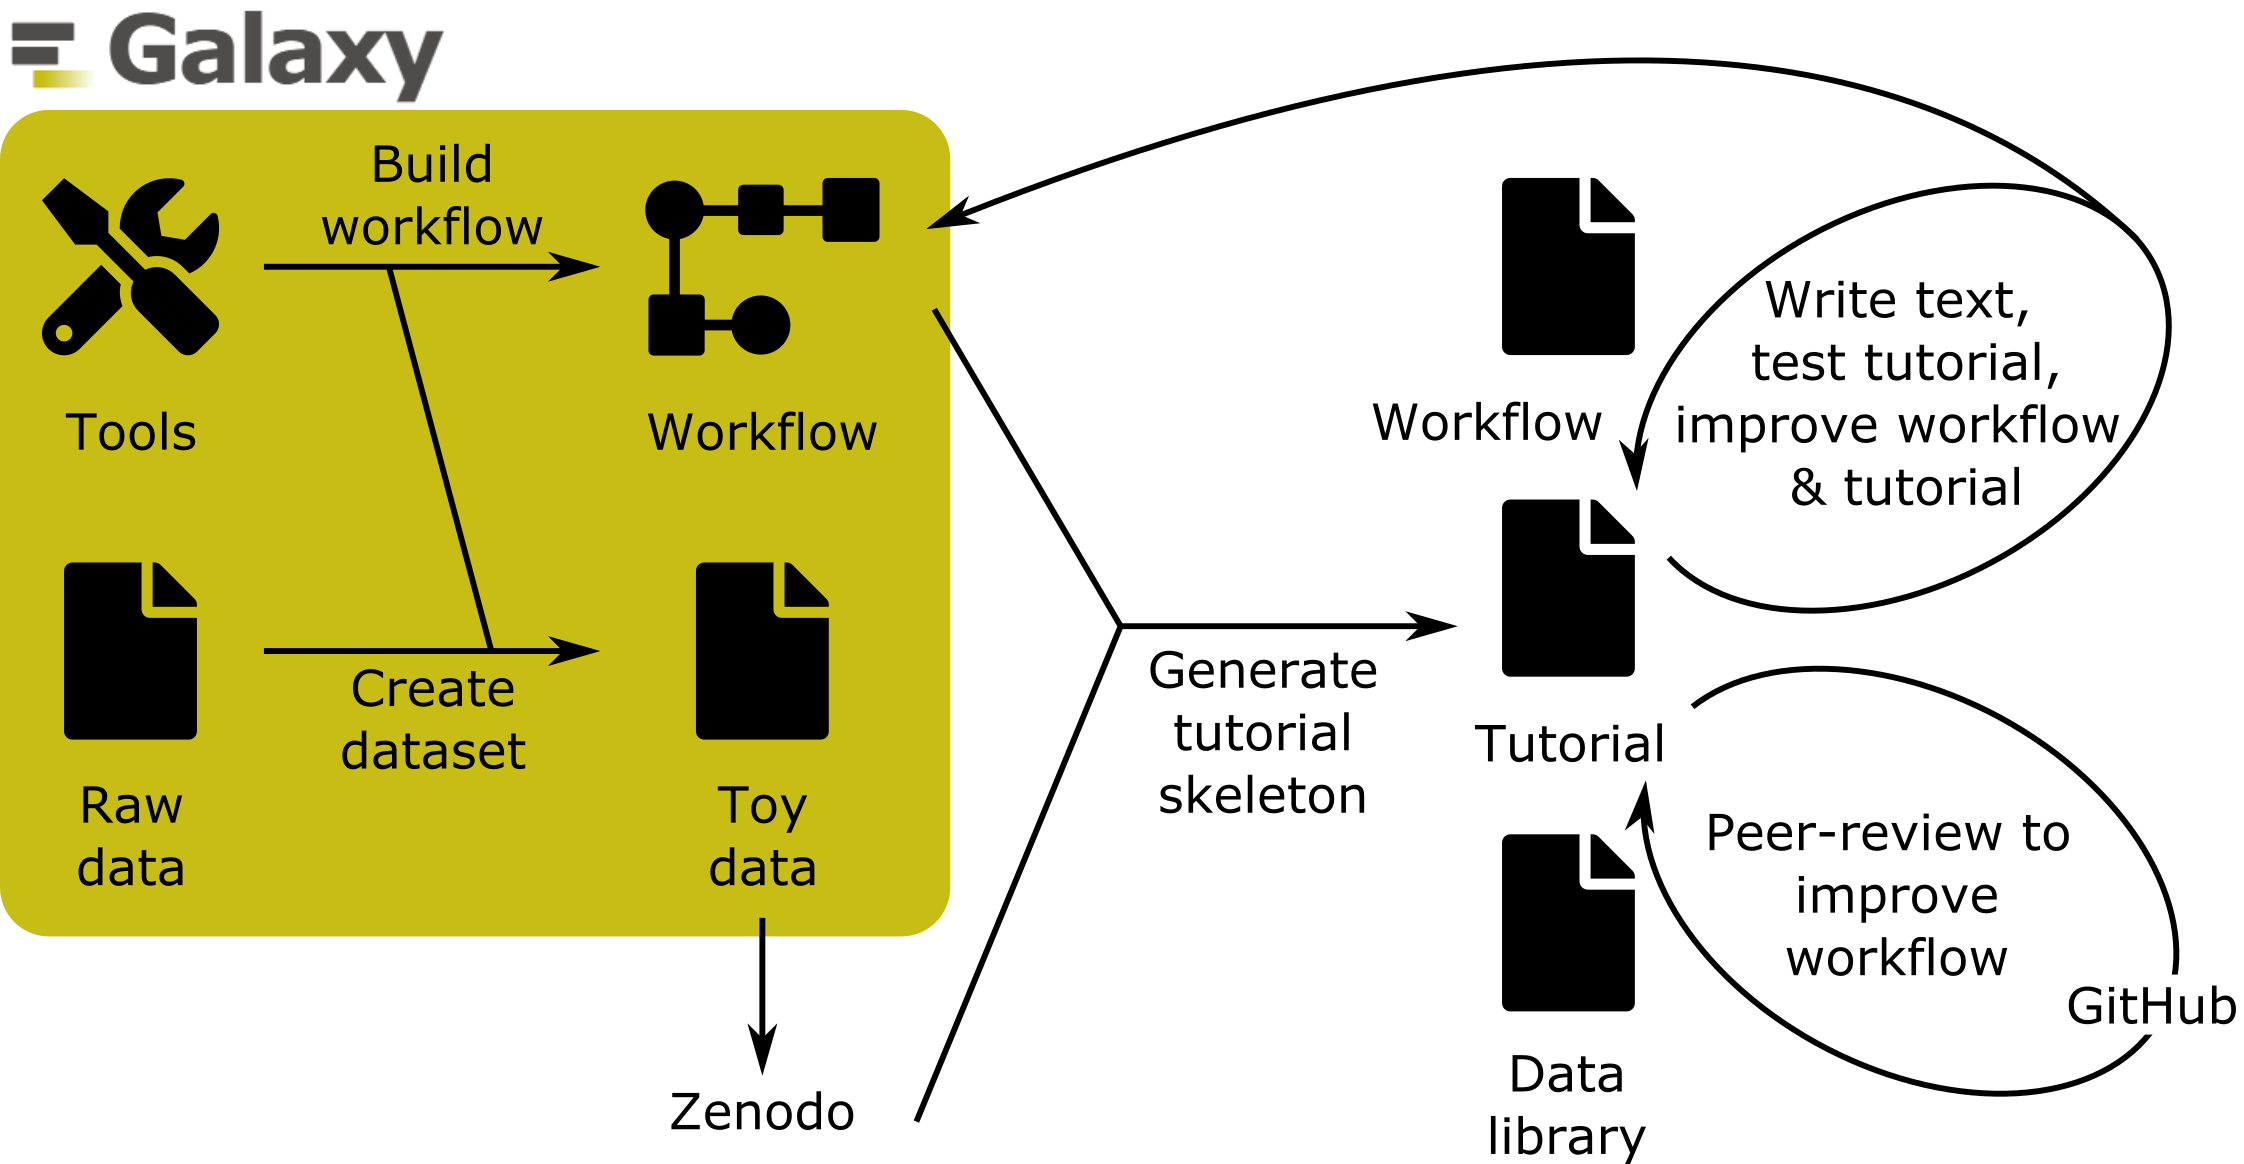
\includegraphics[width=\textwidth]{images/contributing.png}
	\caption{Typical process to create a new tutorial\label{fig:contributing}. Authors usually start by identifying suitable input datasets, and developing the workflow in Galaxy. Thus workflow can be automatically converted into a tutorial skeleton using Planemo's PDTK. The tutorial is then tested, reviewed and finally merged into the GTN.}
\end{figure}


\subsubsection*{Planemo Tutorial Development Kit (PDTK)}

To simplify the tutorial development process, we have created a \emph{Tutorial Development Kit} within the Planemo tool (\url{https://planemo.readthedocs.io}). This automatically generates a tutorial skeleton from a Galaxy workflow as a starting point for tutorial authors.
This skeleton contains the overall structure of the tutorial, including metadata section, auto-generated hands-on boxes for every analysis tool in the workflow, example question boxes for formative assessments, and instructions on how to proceed with adding scientific and pedagogical content. 
This process greatly reduces the development time, and allows tutorial creators to focus on the scientific content of the tutorial, rather than the technical details and style guidelines.

In order to further lower the contribution barrier, this \emph{Planemo Tutorial Development Kit} has been encapsulated into a web service (\url{https://ptdk.herokuapp.com/}), where training material authors can provide a link to a public workflow on one of the UseGalaxy.* servers, and obtain a tutorial skeleton based on this workflow. This removes the need for contributors to install and run Planemo locally. We have found that this approach saves time for not only the contributors but also for reviewers, since the training materials contributed using this method adhere well to the training material’s style guide.

To avoid duplication of content between tutorials, we have developed a set of modular tutorial components, called \emph{snippets}, which can be easily re-used across tutorials.
For example, common tasks in Galaxy such as starting a workflow or creating a new history will be a part of most tutorials. Contributors can include these snippets at any place in a tutorial with a simple import statement. If instructions for this common task change due to e.g. changes in the Galaxy platform, the changes need only be made in the snippet itself, and will automatically propagate to any tutorial using them. 

\subsubsection*{Tutorial Preview and Testing}
GTN tutorials are written in Markdown format for ease of contribution, and subsequently converted to HTML web pages automatically by our framework. In order for contributors to preview the HTML version of their tutorials during development, we offer simple commands to build the GTN website locally on their own machines. Additionally, contributors who do not wish to install and run the GTN locally, can also generate a preview of their in-development tutorials online using GitPod (\url{https://gitpod.io/}). 
We have integrated the GTN GitHub repository with GitPod, enabling contributors to obtain an online tutorial development environment, complete with online preview, with a single click of a button. GitPod has proven particularly useful for collaboration between multiple lesson developers with varying degrees of familiarity with GitHub.    

In addition to a visual inspection of the generated web pages, our framework offers a suite of testing tools, allowing contributors to check that their tutorial meets the technical and style guidelines.
These tests include checks of whether all required metadata is present, whether links within the tutorial are valid, and whether files are correctly formatted.
This helps contributors and reviewers to quickly identify and correct potential problems with a tutorial.


\subsubsection*{Peer Review}

Once a contributor is happy with their tutorial, they can create a \emph{pull request} (PR) to the GTN GitHub repository (\url{https://github.com/galaxyproject/training-material}), where each contribution will then undergo a peer-review process.

This review process is completely open, and any volunteers from the community may participate.
For each topic within the training materials, the GTN has encouraged several prominent community members who are regular contributors to act as topic \emph{maintainers}; maintainers help safeguard the quality of the content in the topic, and are empowered to review, approve, and merge contributions.
Maintainers and other reviewers will check the proposed contribution, both in terms of formatting and scientific content. 
They can make suggestions for updates, and start a discussion with the contributor(s). 
Typically there will be two or three reviewers for any given pull request.
Based on these reviews, the contributor(s) will update the tutorial, and this cycle of update and review will continue until both contributor and reviewer are happy with the result. In case of disagreements, topic maintainers will decide on the path forward.
In order to support peer reviewers, all available quality assurance tests in our framework are automatically run on incoming pull requests, using the GitHub Actions framework.

This open strategy for content creation and updates is paying off.
Since the beginning of the project in the middle of 2016, over 1,500 pull requests have been created to add or update tutorials (Table~\ref{tbl:pullRequestReviewing}).

Thanks to a fast turnaround (on average, it takes \~20 days between the opening of a pull request and its merge), tutorials are regularly updated and iteratively improved over time, keeping the material relevant and of a high quality.
Indeed, each tutorial undergoes (on average) a pull request every month to update it. Some highly used tutorials, like the “Reference-based RNA-seq” tutorial, got around 50 pull requests over the last 3 years, on average one every 3 weeks.

\begin{table}[]
\begin{adjustwidth}{0in}{0in} % Comment out/remove adjustwidth environment if table fits in text column.
	\centering
	\caption{Statistics about Pull Request (PRs) on GitHub repository since 2016.\label{tbl:pullRequestReviewing}}
	\begin{tabular}{l|p{0.15\textwidth}p{0.15\textwidth}p{0.15\textwidth}p{0.15\textwidth}}
 & Number & Reviews and comments per PR (avg) & Reviewers per PR (avg) & Duration per PR (avg) \\\hline
PRs to add tutorial(s)  & 253  & 10.8  & 2.8 & 31 days\\
PRs to update tutorial(s) & 1,286 & 3.3 & 1.7 & 9 days\\
Other PRs & 599 & 2.4 & 1.5 & 5 days\\
	\end{tabular}
\end{adjustwidth}
\end{table}

\subsubsection*{Maintenance \& Feedback}

Tutorials are dynamic entities; underlying analysis tools receive updates, new tools are developed, and the Galaxy interface itself changes regularly.
As a result, tutorials must undergo regular updates as well to reflect the state-of-the-art in the scientific domain, and correctly reflect the latest available version of the tools and the Galaxy interface.

Instructors preparing for their next workshop often check the tutorials as preparation, and in the process identify the places where the tutorial should be updated.
If the instructors feel comfortable making these changes themselves, they can open a pull request proposing the changes.
If not, they can create an \emph{issue} on GitHub to request the changes.

Furthermore, learner feedback is one of the most valuable resources to inform training improvements.
A feedback form is embedded at the end of every tutorial, where users can provide feedback and make suggestions for improvements. 

All feedback received is collected on the GTN website (\url{https://training.galaxyproject.org/feedback}), enabling the community to view and address the feedback (Figure~\ref{fig:feedback}).

\begin{figure}[!ht]
	\centering
	\begin{subfigure}[b]{0.7\textwidth}
         \centering
         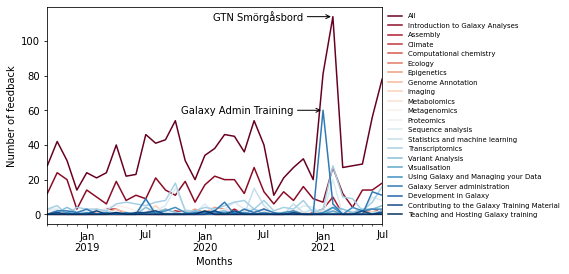
\includegraphics[width=\textwidth]{images/feedback.png}
         \caption{Number of feedback over months}
         \label{fig:feedback-}
    \end{subfigure}
    \hfill
    \begin{subfigure}[b]{0.7\textwidth}
         \centering
         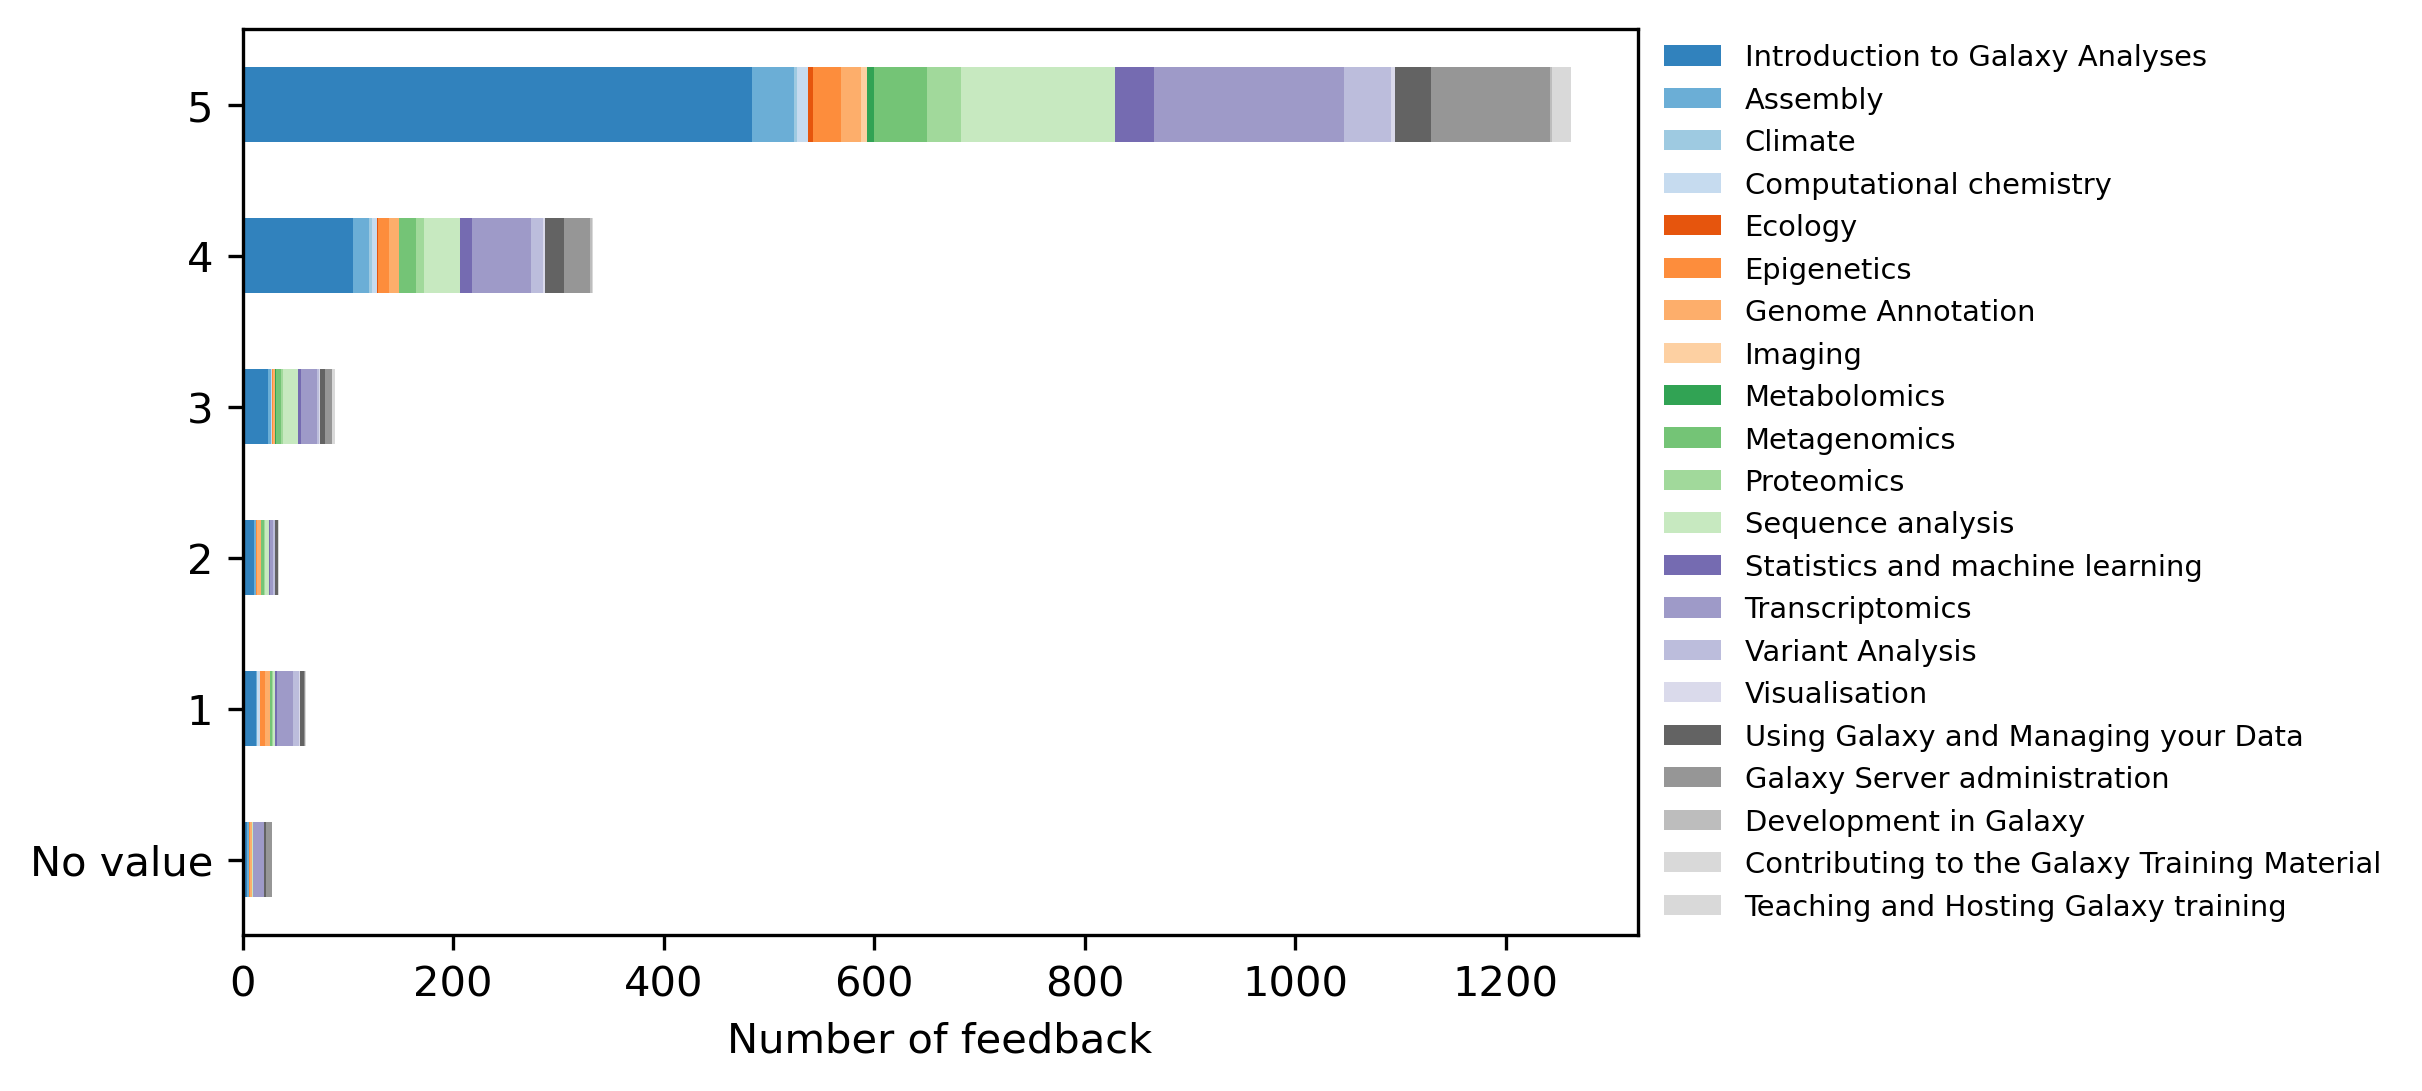
\includegraphics[width=\textwidth]{images/feedback-scores.png}
         \caption{Scores for feedback}
         \label{fig:feedback-scores}
    \end{subfigure}
	\caption{Number and results of the embedded feedback in the tutorials. Three questions are asked in the form: ``How much did you like this tutorial?'' (from 1 (bad) to 5 (great)), ``What did you like?'', ``What could be improved?''. The Jupyter notebook used to create these figures is available on the GitHub repository for this paper (\url{https://github.com/galaxyproject/GTN-community-paper-2020}).
    \label{fig:feedback}}
\end{figure}



%%%%%%%%%%%%%%%%%%%%%%%%%%%%%%%%%%%%%%%%%%%%%
\subsection*{User Stories: GTN across all levels of education}\label{sec:userstories}
%%%%%%%%%%%%%%%%%%%%%%%%%%%%%%%%%%%%%%%%%%%%%


\subsubsection*{GTN in Higher Education}

Galaxy and the GTN are an integral part of Bioinformatics programs at the undergraduate level (e.g. Clermont Auvergne University, Texas A\&M University, Avans Hogeschool, University of Freiburg). 

In these undergraduate courses, Galaxy is often used to teach the concept of pipelines and workflows, and also reproducibility. Students learn the importance of the tool versions, as tools can change subtly or significantly over time and this may impact their analyses. Teachers can likewise showcase the evolution of algorithms over time using different versions of tools (e.g.\ bowtie and bowtie2) to help students understand the advances in the field. 
Without the need to spend resources on teaching basic Unix and command line skills, the time can be fully used to introduce each step (data cleaning, data analysis and visualization) and to go into details of each tool. Galaxy is also convenient to explain how data is structured (data types, metadata), and its connection to tools. Finally, Galaxy can be used to illustrate complete analytical workflows paying attention to input and output data.

Postgraduate courses (e.g. Agrocampus Ouest, Rennes University, Brest University, Clermont Auvergne University, Station Biologique de Roscoff, Melbourne University, University of Freiburg) as well as internal bioinformatics short-format training sessions (e.g. Friedrich Miescher Institute, French Bioinformatics Institute, Erasmus MC, University of Freiburg) are relying on Galaxy as the main teaching tool.

Galaxy is used to introduce the users to classical tools suites and workflows without diving into the command line and scheduling system environment. The focus is on the tools, their parameters and the scientific meaning. These courses are usually directed at scientists who are not comfortable working with the command line. However, we often notice that beginners in bioinformatics like to familiarise themselves with Galaxy as a step towards learning computer languages and working with the command line. After getting familiar with each analysis step and understanding the meaning of parameters of each tool, it is easier to move to command line environments to analyse high throughput data. Thus, it easily allows the course organisers to have both life scientists without any coding skills and users with this knowledge in the same audience.

\subsubsection*{GTN for Research Scientists}

GTN materials are also often used to provide supplemental training to later-career research scientists, for example in the Erasmus Medical Center (EMC). These trainings often consist of short-running workshops, usually aimed at familiarizing researchers with novel analysis techniques. Since many of the GTN tutorials are centered around an analysis pipeline described in a recently published article, they are ideally suited to provide researchers with an update on the latest state-of-the art analysis pipelines in their domain. 
GTN tutorials are also frequently created as part of scientific publications by authors presenting a novel analysis method, as an additional form of documentation for the readers (\cite{Mehta2021, deKoning2020, Tekman2020}).

\subsubsection*{Training in underrepresented communities: Africa as an example}

Reliable internet access is often taken for granted by researchers. Bottlenecks in infrastructure may, however, cause significant issues for bioinformatics training events, as many students try to upload or download data at once. This is especially problematic in low or middle income countries (LMICs) where internet access may be intermittent, restricted or completely unavailable.

Trainers are often brought in from afar, meaning that the teaching takes places in - for the trainer - an unfamiliar setting, and on a strict time schedule limited by the return trip(s) of those involved. It is therefore important to avoid or minimise unforeseen delays caused by incompatibilities with local infrastructure, connectivity failures or unforeseen updates forcing new software to be downloaded or queries to remote servers to fail.

Based on these needs, the eBioKit \cite{Hernandez2017} was developed: it is an assembly of open source or free-for-academic-use software, along with key databases and selected material for bioinformatics. It can be installed beforehand, brought on a portable server to the local training, and made available on the local network. Students can then access it through the network and work directly on the server, which avoids installation issues for the students, unforeseen updates of web services, or other failures. Galaxy has been a part of the eBioKit for most of its existence, specially in the eB3Kit which includes a Galaxy-based bioinformatics platform with a specialised workflow interface \cite{Klingstrom_2017}. %%Docker images of Galaxy, such as the ones provided for training, can easily be installed in a plug and play manner on the eBioKit or eB3Kit.

Various versions of the eBioKit has been used for over a decade by organisations such as EMBnet, H3Abionet, SANBio, and BECA/ILRI to train hundreds of researchers and bioinformatics trainers in LMICs.

TIaaS is also a valuable tool for training in LMICs with limited internet access. All input datasets used in GTN tutorials reside either on the Galaxy server itself, in a \emph{shared data library}, or in a third-party service such as Zenodo. When learners import these datasets into Galaxy provided via TIaaS, their own (poor) internet connections are bypassed for these bandwidth-heavy tasks, and the user's internet is only used to monitor the progress of the analysis in Galaxy. 

For cases where internet access is frequently absent, the GTN offers Docker \cite{Boettiger2015} images, allowing for completely offline training. Every topic has its own Docker image, preconfigured with all the necessary tools, workflows, tours and data-libraries to complete the tutorials within that topic. Drawback of this solution is that all required compute resources to complete the tutorials must be available locally. 


\subsubsection*{Citizen science and education}

Thanks to the graphical user interface, Galaxy can also be used to introduce bioinformatics to a general audience and include them into scientific projects.

The Street Science Community (\url{https://streetscience.community}) offers workshops to introduce biology, genomic sciences and bioinformatics to the public. For exemple, participants extract yeast DNA out of beer bottles and sequence it using the MinION, the Oxford Nanopore sequencing device. The generated sequencing data are then processed by participants inside Galaxy: uploading data, running a metagenomic analysis workflow, and visualizing results. Combining lab work and bioinformatics data analysis with Galaxy vividly demonstrates the challenges and possibilities that genomics brings to our society.

Galaxy has also provided an opportunity for the ecology community to experiment several ways to extend citizen science schemes, for instance, through two monitoring schemes from Vigie-Nature (\url{https://www.vigienature.fr/}), French citizen science programs about common birds (ref STOC) and bats (ref Vigie-Chiro). Volunteers may use Galaxy to analyze data they gathered as researchers would do through user-friendly tools and workflows. Such solutions increases the motivation of participants, specially volunteers, as they can analyze, visualize data about species and ecological systems they monitor, sometimes for several years, and then is increased by such solutions to visualize and analyze their data as they often originally volunteer to discover and increase their knowledge about the species and ecological communities they monitor.
The Vigie-Nature program also coordinates a scheme destined to pupils from primary to high school, Vigie-Nature Ecole (\url{https://www.vigienature-ecole.fr/}), which handles the Galaxy instance Galaxy-Bricks (\url{https://bricks.vigienature-ecole.fr/}). Galaxy-Bricks intends to help teachers and their students understand how does an ecological analysis takes place, from the early stages of formulating a consistent question to a final conclusion drawn from proper statistical tests. This instance gives access to the whole data collection gathered by schools involved in the Vigie-Nature Ecole scheme enabling pupils to perform analyzes on a broader scale.
Based on the Massively Open Online Data Analysis concept (MOODA, ref) and in collaboration with SPIPOLL (ref), a crowd sourcing interface has been implemented to Galaxy for users to participate during loading time. Pictures of marmalade hoverflies are displayed one by one and the user has to identify the sex of the individual based on the size of the gap between its eyes. This initiative has permitted to register more than 23 000 classifications in 2020.

\subsubsection*{Training in the COVID-19 era: Remote Learning}
Due to the global COVID-19 pandemic, many educators have found themselves forced to change the modality of their training activities to completely virtual events.
Galaxy and the GTN cater to remote learners and teachers with a set of features to facilitate the online learning process. It provides easy access to data and the possibility to share the progress and achievements, both student-to-student and student-to-instructor \cite{SerranoSolano2020}. This has been extensively tested during the COVID-19 pandemic. For example, Galaxy Europe held a 5-day workshop on ``Machine Learning using Galaxy'' in June 2020, with 400+ registrations and 200+ participants on the first day \cite{FreiburgGalaxyTeam2020}. The main goal of the workshop was to introduce machine learning using Galaxy to researchers at any career stage, by combining webinars and self-study sessions. The webinar sessions aimed to introduce machine learning and how those methods can be applied using Galaxy. After each webinar session, there was a self-training day, in which the attendees could follow the tutorials themselves and ask questions to the experts in a support channel.

As a second example, the GTN organized the GTN Smörgåsbord event, a global, 5-day, 24/7 event. This was a fully asynchronous event, where instructors pre-recorded GTN tutorials, which participants could work through at their own pace, with over 60 instructors available online for support in all time zones.

\subsubsection*{Hybrid learning in geographically sparse locations} 
Even before the pandemic, learners in remote areas have faced significant barriers to travelling to in-person training events. In such areas, a so-called \emph{hybrid training} approach may offer a solution. In such an approach, learners gather in classrooms in several geographically distinct locations. The training is live-broadcast to each of these locations, and communication with the instructor happens in real-time. 
GTN resources have been successfully used for such hybrid training events, for example by Galaxy Australia, which organized a large number of hybrid training events, with up to 11 satellite classrooms across the region participating, and reaching over 800 learners \cite{Hall2021}. The Gallantries project (\url{https://gallantries.github.io/}) has successfully applied a similar aproach in the European region.

\section*{Conclusion}

From the start of the Galaxy project, education has been an important focus. Offering training as part of conferences or in the form of dedicated workshops has helped to grow and foster the worldwide Galaxy community and has brought (biological) data analysis to a broad audience. Much training material has been collected and made available on the Galaxy project website. In its original form, the collection lacked a proper structure, and most of those ad-hoc assembled materials became out-of-date soon after publication.

The Galaxy Training Network has created the Galaxy Training Platform. It is maintained in GitHub and has made it possible to coordinate and structure all those previous efforts in a sustainable way. It makes it easy to manage the addition of new tutorials and/or updating existing ones. Additionally, efforts have been directed to build a powerful training infrastructure while keeping contribution barriers as low as possible. Thus, it has become a valuable resource for the trainees, the instructors and the developers of training content.

Given the feedback from learners, instructors and contributors, new features are currently in development. We are extending efforts to integrate videos to support the slides, but also videos to show some specific aspects of Galaxy interface. To avoid the cumbersome aspect of the updating these videos, we are developing a framework to generate and update them automatically.
In the instructor survey, the trainers have been asked about the improvement they wished to see in the GTN resources. One of the concerns is the access to computational resources, such as using public instances, or having backup servers if the server dedicated to the workshop encounters a problem.
Another important need is the access to GTN material metadata, such as: what new version of training has been published, what new training subject could require contributors. Users suggest that the pedagogic value of training materials could be improved by directing the users to different training depending on their level of expertise, and to provide more context to the analyses.
Some trainers would like more interactivity with the tutorials through exercises or through facilitating the parallel between the tutorial and the Galaxy instance. We plan to answer these suggestions by implementing them. 
To support the instructors and build a community of instructors, we are also implementing with the Gallantries project and in collaboration with ELIXIR, a Train the Trainer program and a mentoring program for instructors. For contributors, we are also working with editors to implement a system for publication of each tutorial via article with limited extra work.

The Galaxy Training Network aims to continue its effort in developing and maintaining this powerful training framework.


\bibliography{references}


\clearpage
\section*{Supplementary Materials}

\subsection*{Figure S1: Analytics of the GTN website}

\begin{figure}[!ht]
    \centering
    \begin{subfigure}[b]{0.45\textwidth}
         \centering
         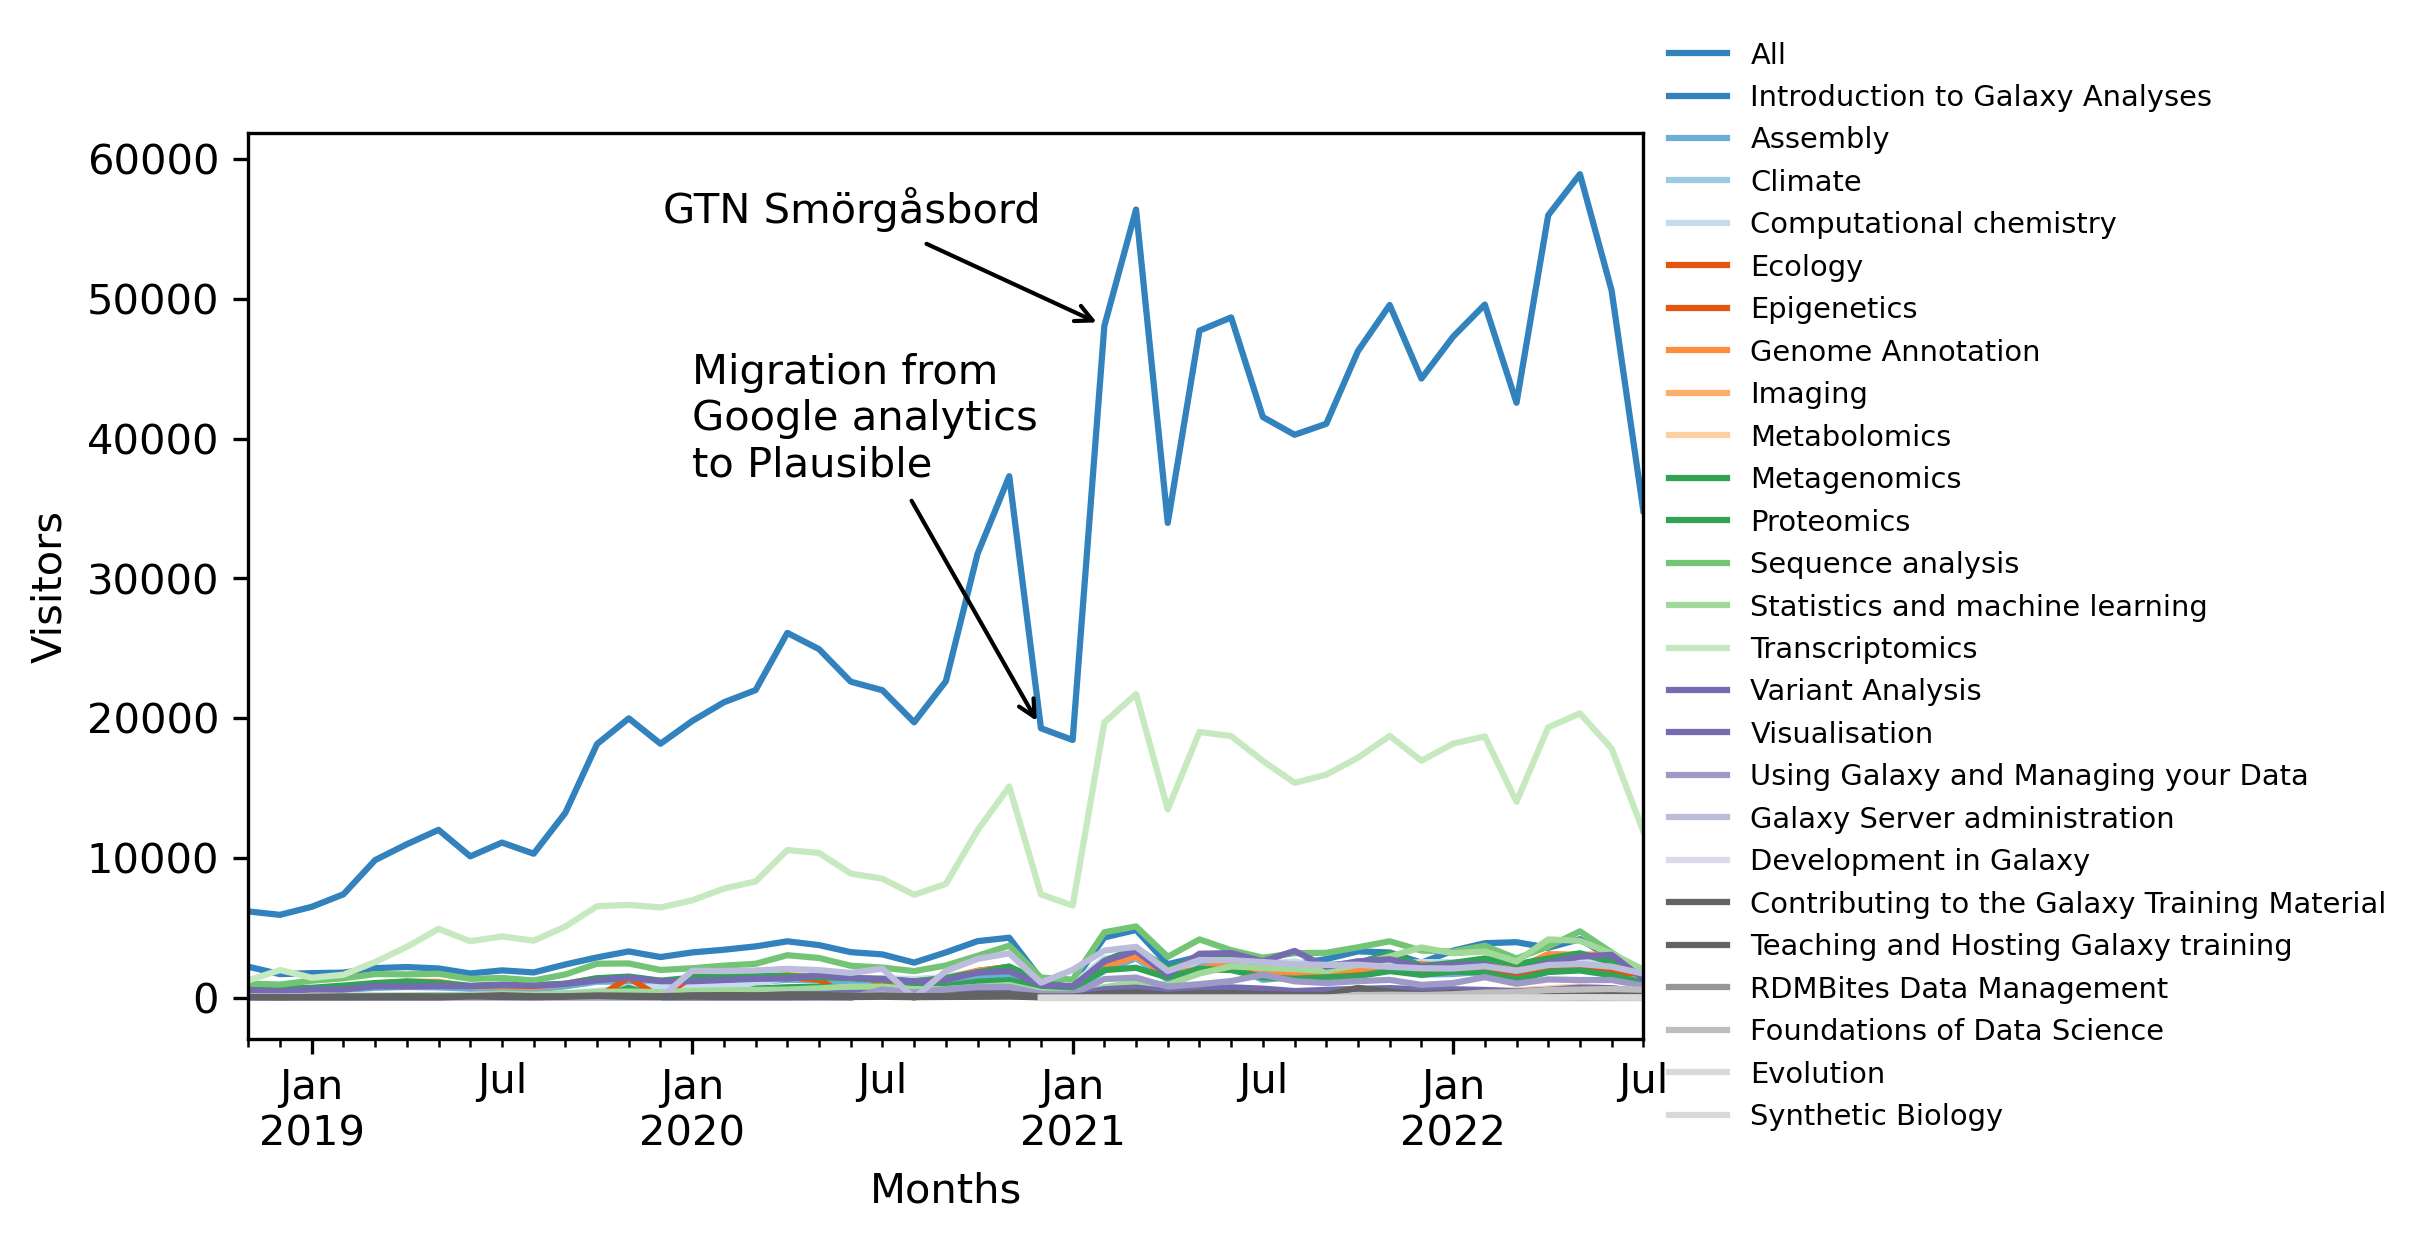
\includegraphics[width=\textwidth]{images/analytics-all-users.png}
         \caption{Number of users per months}
         \label{fig:analytics-all-users}
    \end{subfigure}
    \hfill
    \begin{subfigure}[b]{0.45\textwidth}
         \centering
         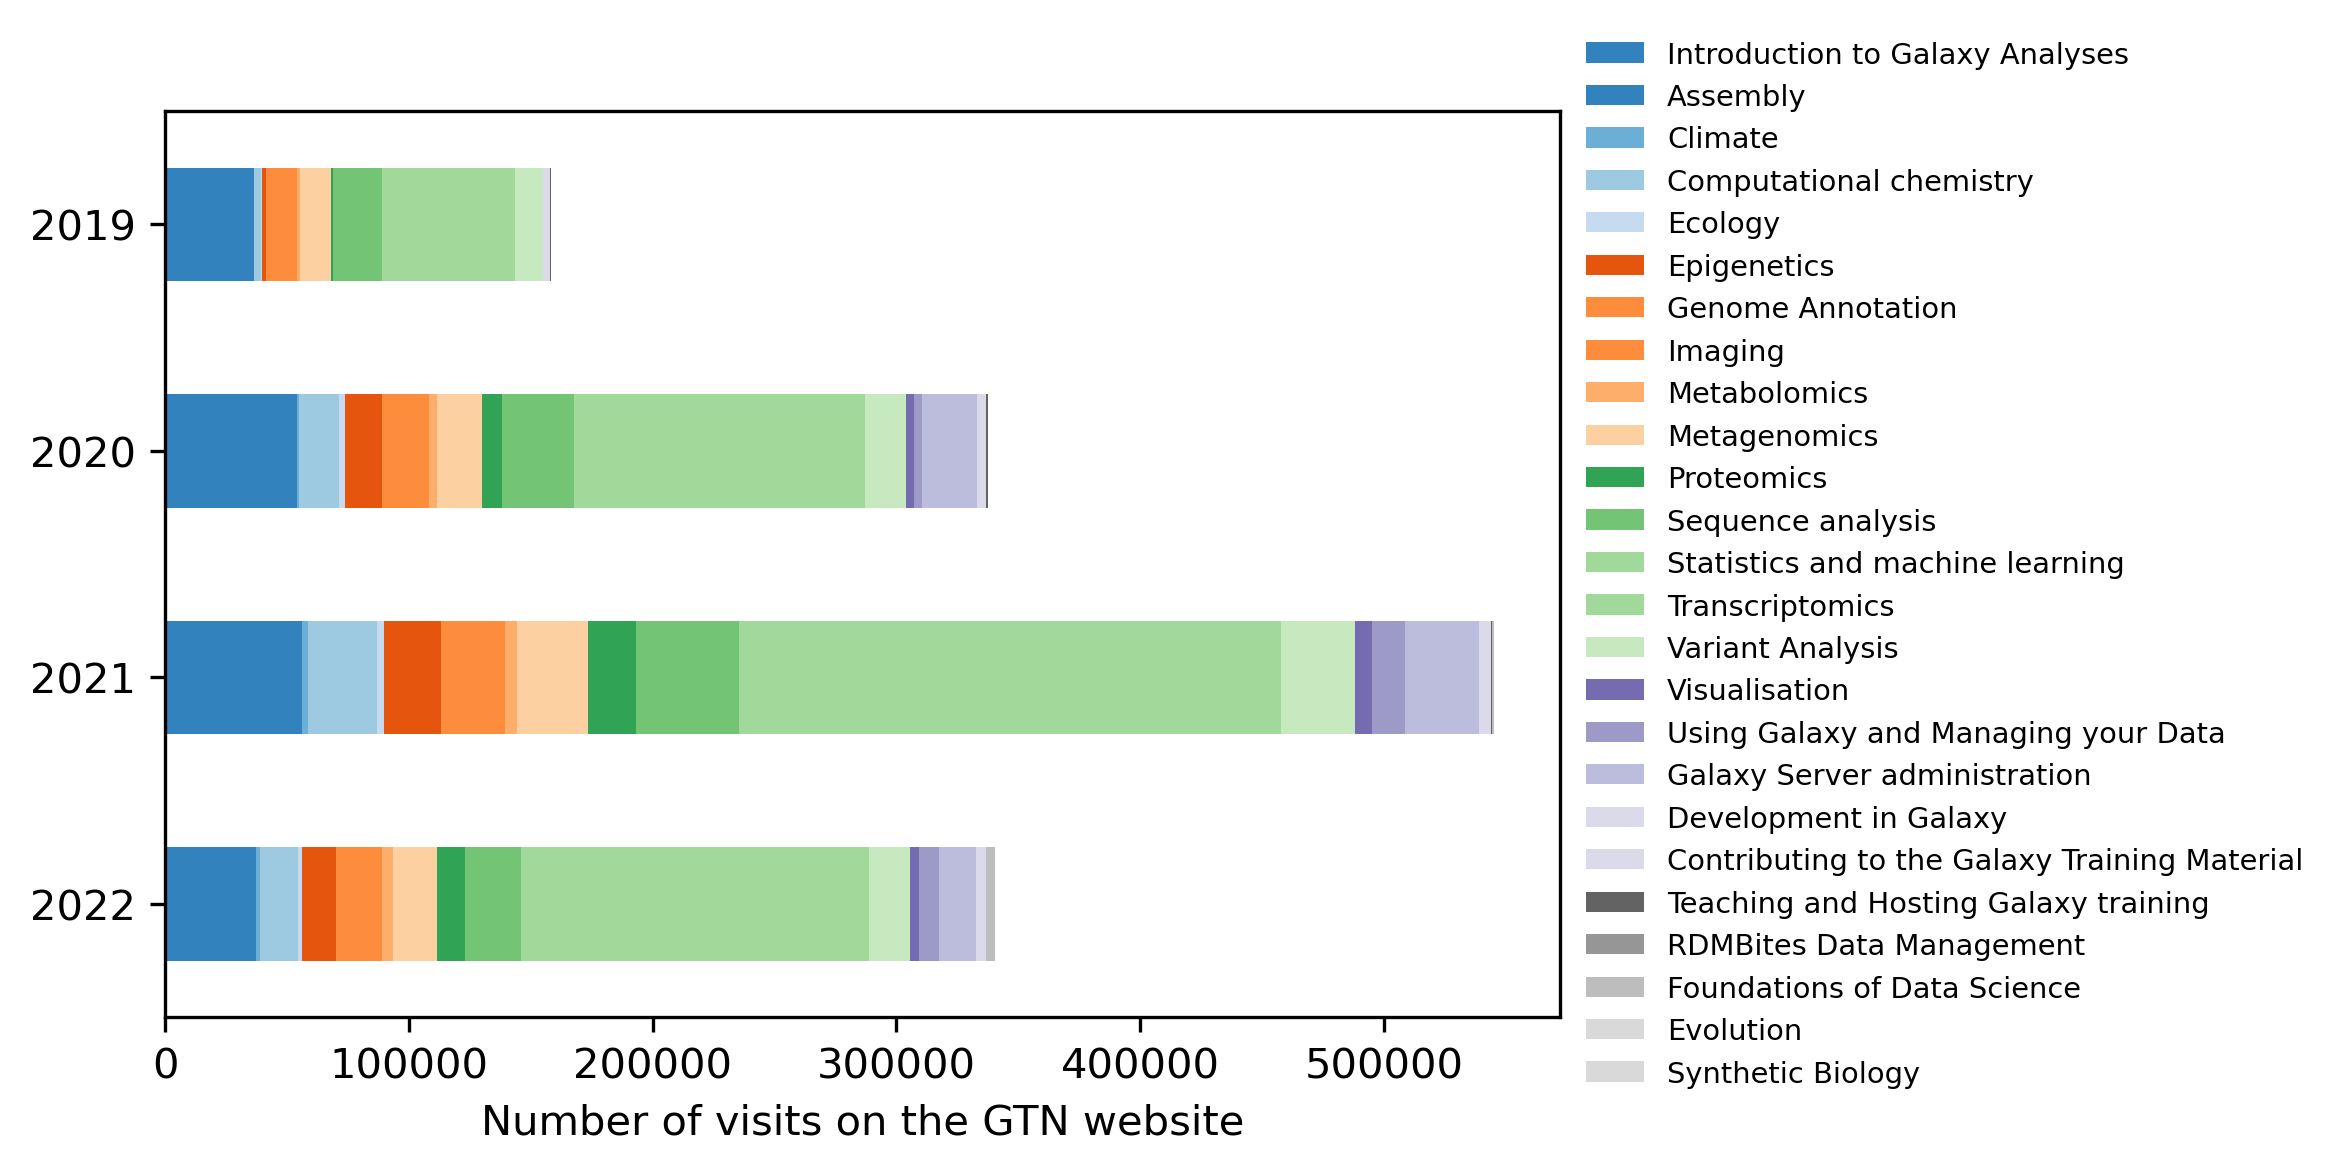
\includegraphics[width=\textwidth]{images/analytics-topics-users.png}
         \caption{Number of users per topics}
         \label{fig:analytics-topics-users}
    \end{subfigure}
	\caption{Number of visits per month on the GTN website \url{http://training.galaxyproject.org/} tracked by Google Analytics and later Plausible. There is a steady growth in usage over time. A dip in visits is visible due to missed data when switching analytics platforms, and large training events such as the GTN Smörgåsbord lead to clear jumps in usage, also beyond the duration of the event itself. 
	The latest usage statistics are publlicly available from \url{https://plausible.galaxyproject.eu/training.galaxyproject.org}, and the Jupyter notebook used to create these figures is available on the GitHub repository for this paper (\url{https://github.com/galaxyproject/GTN-community-paper-2020}).}
	\label{fig:visits}
\end{figure}

\clearpage
\subsection*{Table S1: Ten Simple Rules}
\begin{table}[!ht]
    \begin{adjustwidth}{-2in}{0in}
	\centering
	\caption{Implementation of the ``Ten simple rules for collaborative lesson development''\cite{Devenyi_2018} in the training material
    \label{tbl:tensimplerules}}
	\begin{tabular}{p{0.5\textwidth}p{0.5\textwidth}}
		\textbf{Rules}                                      & \textbf{Implementation in the GTN framework} \\
		Clarify audience                                    & Tutorial metadata includes level indicators (introductory, intermediate, advanced) and a list of prerequisite tutorials as recommended prior knowledge. This information is rendered at the top of each tutorial. \\
		Make lessons modular                                & Development of small tutorials linked together via learning paths \\
		Teach best practice lesson development              & A topic \emph{Contributing to the Galaxy Training Material} including 10 tutorials describing how to create new content. Furthermore, quarterly online collaboration fest (CoFests) are organized, where contributors can get direct support. Development of a Train the Trainer program and a mentoring program for instructors, in which lesson development is taught \\
		Encourage and empower contributors                  & Involve them in reviews. Mentor them. Encourage them to become maintainers. \\
		Build community around lessons                      & Quarterly online collaboration fest (CoFests) and Community calls. Chat (Gitter channel) \\
		Publish periodically and recognize contributions    & Author listed on tutorials. Hall of fame listing all contributors. Full tutorial citation at the end of the tutorial. Tweet about new or updated tutorials. List of new or updated tutorials in Galaxy Community newsletter. Soon: publication of tutorials via article \\
		Evaluate lessons at several scales                  & Tutorial change (Pull Request) review. Embedded feedback form in tutorials for trainee feedback. Instructor feedback. Automatic workflow testing \\
		Reduce, re-use, recycle                             & Sharing content between tutorials, specially using snippets. Development of small modular tutorials linked by learning paths \\
		Link to other resources                             & Links to original paper, documentation, external tutorials and other material \\
		You can't please everyone                           & but we can try (several different Galaxy introduction tutorials for different audience). Aim to clearly state what the tutorial does and does not cover, at the start.  \\
	\end{tabular}
	\end{adjustwidth}
\end{table}

\clearpage
\subsection*{Table S2: 10 Simple Fair Rules}
\begin{table}[h!]
    \begin{adjustwidth}{-2in}{0in}
	\centering
    \caption{Implementation of the ``10 simple rules for making training materials FAIR'' \cite{Garcia2020} in the GTN training material framework
    \label{tbl:rulesforfair}}
	\begin{tabular}{p{0.4\textwidth}p{0.6\textwidth}}
		\textbf{Rules}                                                                & \textbf{Implementation in GTN framework}\\\hline
		Plan to share your training materials online                                  & Online training material portfolio (\url{https://training.galaxyproject.org/}), managed via a public GitHub repository (\url{https://github.com/galaxyproject/training-material})\\
		Improve findability of your training materials by properly describing them    & Rich metadata associated with each tutorial that are visible and accessible via schema.org on each tutorial webpage\\
		Give your training materials a unique identity                                & URL persistency with redirection in case of renaming of tutorials.
		Data used for tutorials stored on Zenodo and associated with a Digital Object Identifiers (DOI) \\
        Register your training materials online                                       & Tutorials automatically registered on TeSS, the ELIXIR's Training e-Support System (\url{https://tess.elixir-europe.org/})  \\
        If appropriate, define access rules for your training materials               &	Online and free to use without registration \\
        Use an interoperable format for your training materials                       &	Content of the tutorials and slides written in Markdown. Metadata associated with tutorials stored in YAML, and workflows in JSON\\
		Make your training materials (re-)usable for trainers                          & Online. Rich metadata associated with each tutorial: title, contributor details, license, description, learning outcomes, audience, requirements, tags/keywords, duration, date of last revision. Strong technical support for each tutorial: workflow, data on Zenodo and also available as data libraries on UseGalaxy.*, tools installable via the Galaxy Tool Shed, list of possible Galaxy instances with the needed tools. (Figure \ref{fig:tutorial-skeleton})\\
		Make your training materials (re-)usable for trainees                          & Online and easy to follow hands-on tutorials. Rich metadata with ``Specific, Measurable, Attainable, Realistic and Time bound'' (SMART) learning outcomes following Bloom's taxonomy. Requirements and follow-up tutorials to build learning path. List of Galaxy instances offering needed tools, data on Zenodo and also available as data libraries on UseGalaxy.*. Support chat embedded in tutorial pages. (Figure \ref{fig:tutorial-skeleton})\\
		Make your training materials contribution friendly and citable                & Open and collaborative infrastructure with contribution guidelines, a CONTRIBUTING file and a chat. Details to cite tutorials and give credit to contributors available at the end of each tutorial (Figure \ref{fig:tutorial-skeleton}).\\
		Keep your training materials up-to-date                                       & Open, collaborative and transparent peer-review and curation process. Short time between updates (Table \ref{tbl:pullRequestReviewing})\\
	\end{tabular}
	\end{adjustwidth}
\end{table}

\paragraph{Figure SX: TIaaS Stats}

\begin{figure}[!ht]
    \centering
    \begin{subfigure}[b]{0.45\textwidth}
         \centering
         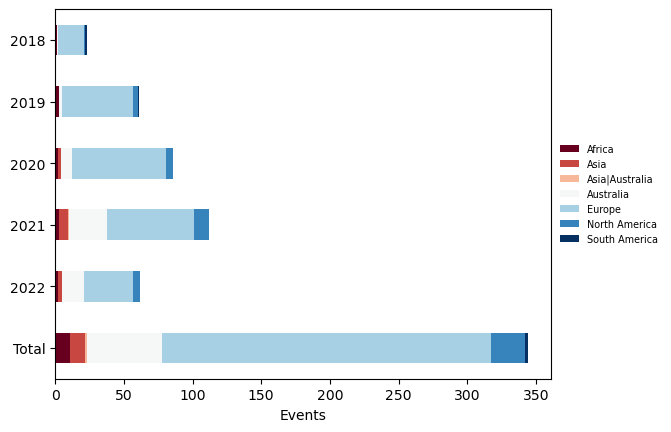
\includegraphics[width=\textwidth]{images/tiaas-events-per-year.png}
         \caption{Events per year and continent}
         \label{fig:tiaas-events-per-year}
    \end{subfigure}
    \hfill
    \begin{subfigure}[b]{0.45\textwidth}
         \centering
         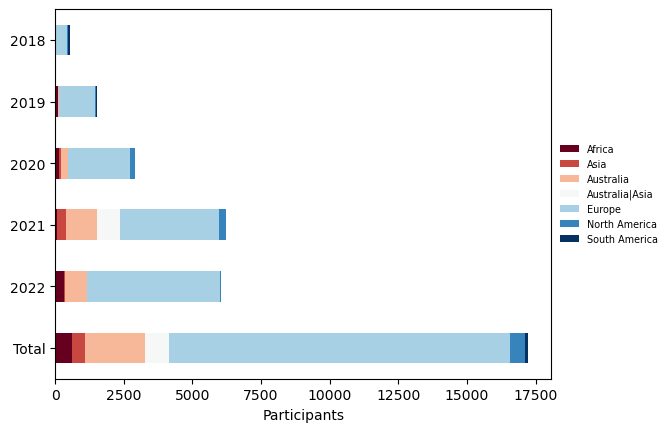
\includegraphics[width=\textwidth]{images/tiaas-participants-per-year.png}
         \caption{Participants per year and continent}
         \label{fig:tiaas-participants-per-year}
    \end{subfigure}
    \hfill
    \begin{subfigure}[b]{0.45\textwidth}
         \centering
         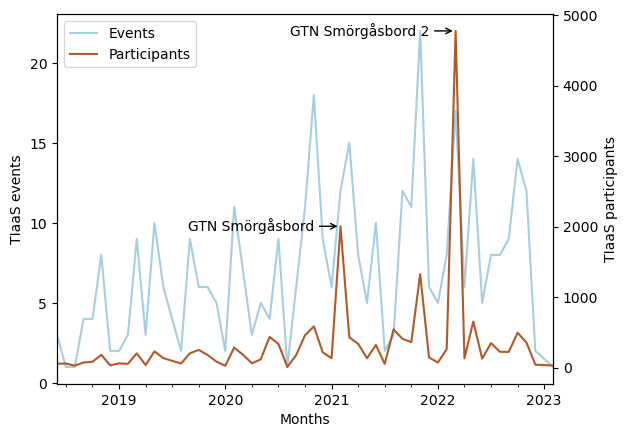
\includegraphics[width=\textwidth]{images/tiaas-events.png}
         \caption{Events and participants over months}
         \label{fig:tiaas-events}
    \end{subfigure}
	\caption{Usage of the TIaaS (Training Infrastructure as a Service) from the European Galaxy server over the months.}. 
	\label{fig:tiaas}
\end{figure}

\end{document}



